\documentclass[tikz]{standalone}
\usetikzlibrary{arrows,shapes,automata,petri,positioning}

\tikzset{
	place/.style={
		circle,
		thick,
		draw=blue!75,
		fill=blue!20,
		minimum size=6mm,
	},
	transitionH/.style={
		rectangle,
		thick,
		fill=black,
		minimum width=8mm,
		inner ysep=2pt
	},
	transitionV/.style={
		rectangle,
		thick,
		fill=black,
		minimum height=8mm,
		inner xsep=2pt
	}
}

\begin{document}
	
	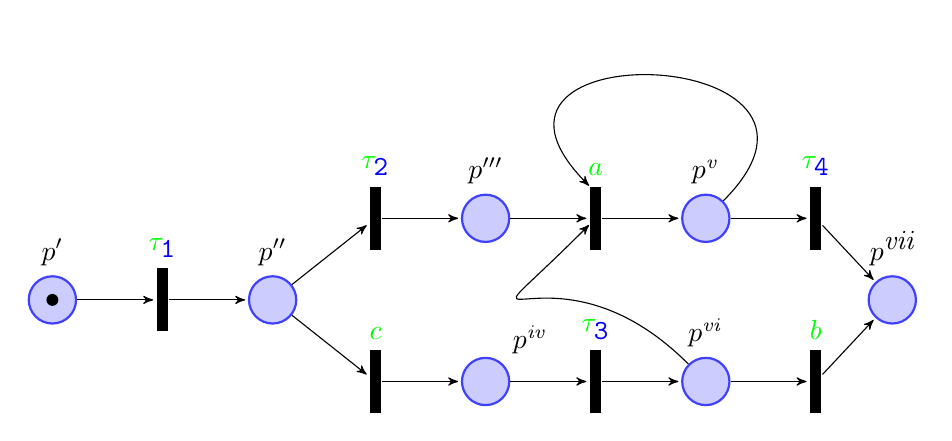
\begin{tikzpicture}[node distance=0.4cm and 1cm,>=stealth',bend angle=45,auto]
	\node [place,label=above:$p^\prime$,tokens=1] (p1) {};
	\node [transitionV,label=above:$\color{green}\tau_\texttt{\color{blue}1}$] (t1) [right= of p1] {} edge[pre] (p1);
	\node [place,label=above:$p''$] (p2) [right=of t1] {} edge[pre] (t1);
	\node [transitionV,label=above:$\color{green}\tau_\texttt{\color{blue}2}$] (eplus) [above right=of p2] {} edge[pre] (p2);
	\node [place,label=above:$p'''$] (pk) [right=of eplus] {} edge[pre] (eplus);
	\node [transitionV,label=above:$\color{green}a$] (a) [right=of pk] {} edge[pre] (pk);
	\node [place,label=above:$p^\mathit{v}$] (p3) [right=of a] {} edge[pre] (a);
	\node [transitionV,label=above:$\color{green}\tau_\texttt{\color{blue}4}$] (e4) [right=of p3] {} edge[pre] (p3);
	\draw[->] (p3.north east) .. controls +(2,2) and +(-2,2) .. (a.north west);
	\node [transitionV,label=above:$\color{green}c$] (e2) [below right=of p2] {} edge[pre] (p2);
	\node [place,label=above right:$p^\mathit{iv}$] (p4) [right=of e2] {} edge[pre] (e2);
	\node [transitionV,label=above:$\color{green}\tau_\texttt{\color{blue}3}$] (e3) [right=of p4] {} edge[pre] (p4);
	\node [place,label=above:$p^\mathit{vi}$] (p6) [right=of e3] {} edge[pre] (e3);
	\draw[->] (p6) .. controls +(-2,2) and +(-2,-2) .. (a);
	\node [transitionV,label=above:$\color{green}b$] (b) [right=of p6] {} edge[pre] (p6);
	\node  (b1) [right=of p2] {};
	\node  (b2) [right=of b1] {};
	\node  (b3) [right=of b2] {};
	\node  (b4) [right=of b3] {};
	\node  (b5) [right=of b4] {};
	\node [place,label=above:$p^\textit{vii}$] (b4) [right=of b5] {} edge[pre] (e4) edge[pre] (b);

	
%	
%	\node [place,label=above:$p_2$] (p2) [above right= of t1] {} edge[pre] (t1);
%	\node [transitionV,label=above:$t_2$] (t2) [above right= of p2] {} edge[pre] (p2);
%	\node [place,label=above:$p_3$] (p3) [right= of t2] {} edge[pre] (t2);
%	\node [transitionV,label=above:$t_4$] (t4) [right= of p3] {} edge[pre] (p3);
%	\node [transitionV,label=above:$t_5$] (t5) [below right= of p2] {} edge[pre] (p2);
%	\node [place,label=above:$p_5$] (p5) [below right= of t1] {} edge[pre] (t1);
%	\node [transitionV,label=below:$t_3$] (t3) [right= of p5] {} edge[pre] (p5);
%	\node (b1) [right = of p2] {};
%	\node (b2) [right = of b1] {};
%	\node (b3) [right = of b2] {};
%	\node [place,label=above:$p_4$] (p4) [right= of b3] {} edge[pre] (t4) edge[pre] (t5);
%	\node (b1) [right = of t3] {};
%	\node (b3) [right = of b1] {};
%	\node [place,label=above:$p_6$] (p6) [right= of b3] {} edge[pre] (t3);
%	\node (b1) [right = of t5] {};
%	\node (b2) [right = of b1] {};
%	\node (b3) [right = of b2] {};
%	\node [transitionV,label=below:$t_6$] (t6) [right= of b3] {} edge[pre] (p4) edge[pre] (p6);
%	\node [place,label=above:$p_7$] (p7) [right= of t6] {} edge[pre] (t6);
%	
	\end{tikzpicture}
	
\end{document}